% !TEX root = ./Thesis.tex
\chapter{NMR theory}

Nuclear magnetic resonance (NMR) theory can be described using two approaches:
\begin{enumerate}
  \item The classical approach, in which the the nuclei are thought of as small bar magnets which
  rotate in 3D space. Experiments can be described be approxiamating the net magnetisation as a
  vector in 3D space.
  \item The quantum mechanical approach, in which each spin in the system is in a distinct quantised state.
  Operators are used to describe the state of a system as a whole. Experiments are described by propagating
  these operators.
\end{enumerate}

The theory described in this chapter is mainly from \citep{RN135,RN136} and is intended to provide sufficient background
knowledge in order for the reader to understand later chapters.

\section{Classical NMR}

\subsection{Spin}

Nuclei, often modelled as a clump of neutrons and protons surrounded by electrons at
the centre atoms, have a property reffered to as spin.

In fact, nuclear spin is an intrinsic property of the nucleus and can take half or whole
integer values, including $0$. In this thesis we will be mainly concerned about one spin-
1/2 nucleus, the proton ($\ce{^{1}H}$), with another spin-1/2 nucleus \ce{^{13}C} making
sparse appearences. Just like in this thesis, $\ce{^{13}C}$ only has an $\approx{1}\%$
abundance in nature with the other $\approx{99}\%$ $\ce{^{12}C}$ having a spin-$0$
nucleus.

All spin-1/2 nuclei possess a magnetic dipole moment and behave rather like small bar magnets in that, when placed in an external magnetic field they have a tendency to align
with the field. In NMR this external field is called $B_0$, and is orientated along the
$z$-axis.

\subsection{Population}

In a magnetic field a spin-1/2 nucles has two energy levels with a separation that is proportional to the strength of the magentic field a schematic is show in \fig{fig:EnergySplit}. We label these levels $\alpha$ and $\beta$.

\begin{figure}
  \begin{center}
  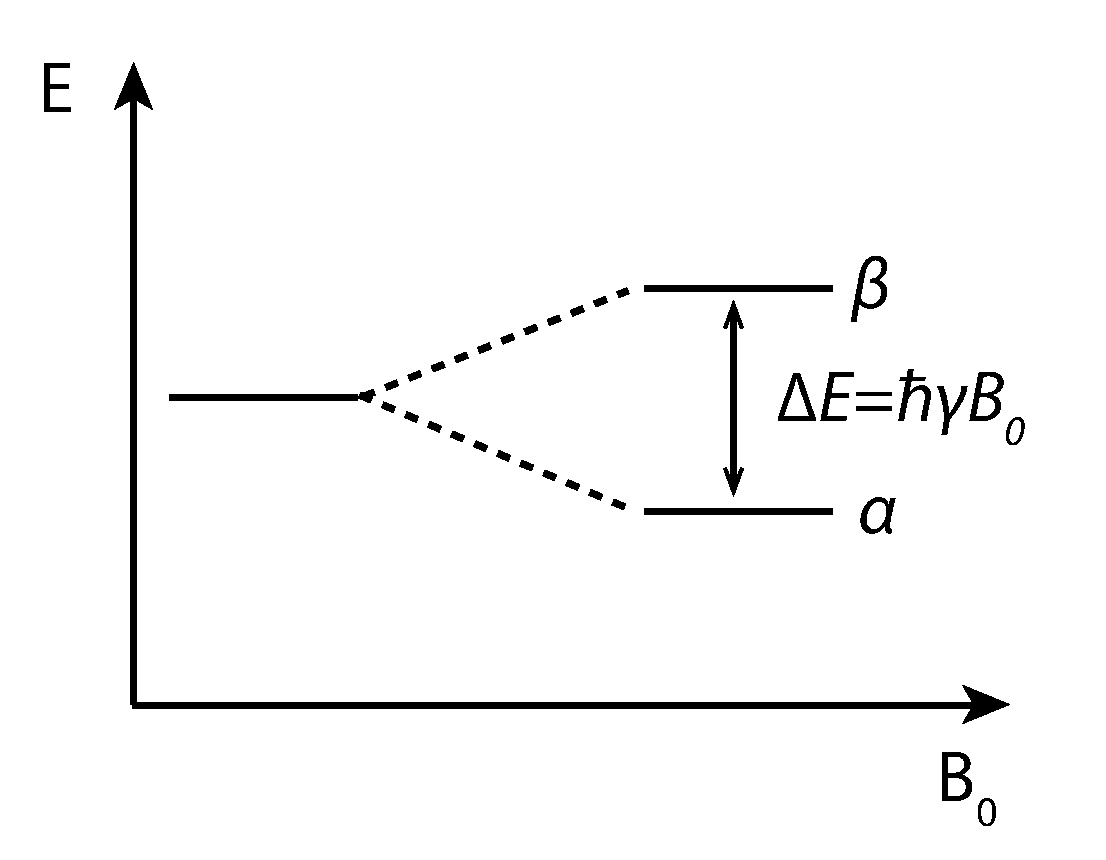
\includegraphics[width=\textwidth,height=5cm,keepaspectratio]{EigenStateLevel.pdf}
  \end{center}
  \caption{Energy level and $\Delta~E$ of the two energy levels for a spin-1/2 nucleus}
  \label{fig:EnergySplit}
\end{figure}

When measuring a group of spins each spin can exist in either the $\alpha$ or $\beta$ state and overall the spins have a slight preference for the lower energy state, $\alpha$. This preference can be quantified by calculating the difference in populations ($P$) which at thermal equilibrium is governed by the Boltzmann distribution:
\begin{equation}\label{eqn:Boltzmann}
  \frac{P_{\beta}}{P_{\alpha}} = \text{exp}\{\frac{-\Delta{E}}{k_B T}\}
\end{equation}

where $P_{\beta}/P_{\alpha}$ is the population ratio between the states, $k_B$ is Boltzmann constant, and $T$ is the temperature. The polarisation, $p$, of a system of
spin-1/2 nuclei is
\begin{equation}
  p = \frac{P_\alpha - P_\beta}{P_\alpha + P_\beta}
\end{equation}

For a system in an NMR experiment which typically operates at 298$K$ and
a field of 14.1$T$ the polarisation level is circa $10^5$ meaning That the spins are aligned weakly in the same direction as the magnetic field. It is this small polarisation that gives rise to the NMR signal and why NMR is famed for sensitivity
issues. One possible solution to this will be described in a later chapter.

\subsection{Nuclear spin precession}

When placed in a magnetic field, the nuclei will precess around the axis of the field at a rate known as the larmour frequency defined as:
\begin{equation}\label{eqn:larmour}
  \omega_j^0 = -\gamma_jB_0
\end{equation}

where $\gamma_j$ is the gyromagnetic ratio for a nucleus, $j$. The gyromagnetic ratio is typically $10$s of MHz $T^{-1}$ that give larmour frequencies in the $100$s of MHz in an NMR experiment.

\subsection{Magnetisation as a vector}

The net magnetic moment of a spin ensemble can be modelled by a 3D vector that can rotates in space. The essence of this is shown in \fig{fig:VectorFig}. Magnetisation is intially taken to be orientated along the $z$-axis, this is called longitudinal magnetisation. It is then rotated into the $xy$-plane which is called transverse
magnetisation that then precesses about the $z$-axis.

\begin{figure}
  \begin{center}
  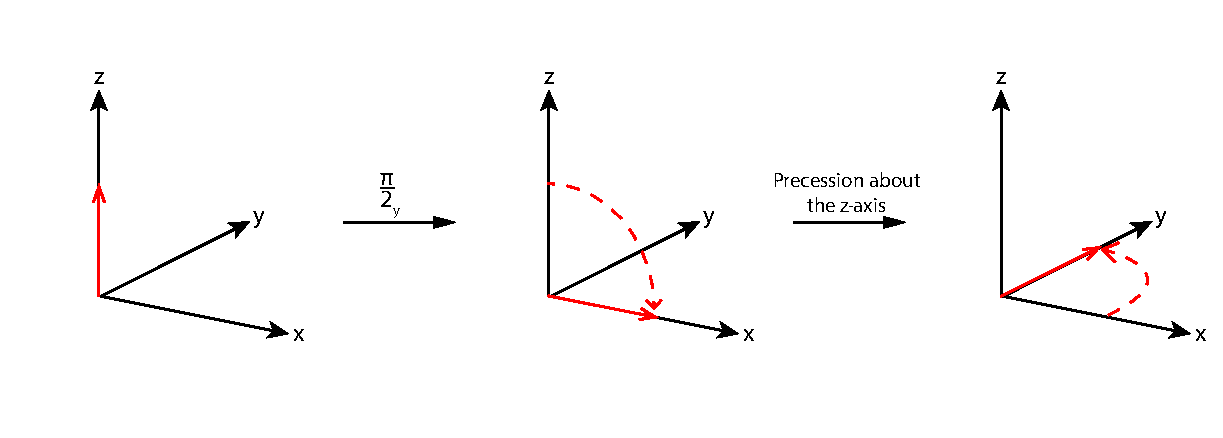
\includegraphics[width=\textwidth]{VectorFig.pdf}
  \end{center}
  \caption{Magnetisation shown as a vector in red, at equilibrium, is orientated on the $z$-axis. A $pi$/2
  pulse rotates the vector to the $xy$-plane where it begins to precess around the $z$-axis.}
  \label{fig:VectorFig}
\end{figure}

How this vector changes in a magnetic field is described using the Bloch equations\citep{Bloch:1946hk}. These are a group of differential equations that
describe how the magnetisation vector components evolves in time in the
presence of orthogonal magnetic fields.
\begin{align}\label{eqn:Bloch}
  \frac{dM_x(t)}{dt}\quad=\quad\gamma(M_y(t)B_z(t)-M_z(t)B_y(t))\\
  \frac{dM_y(t)}{dt}\quad=\quad\gamma(M_z(t)B_x(t)-M_x(t)B_z(t))\\
  \frac{dM_x(t)}{dt}\quad=\quad\gamma(M_x(t)B_y(t)-M_y(t)B_x(t))
\end{align}
where $M_a$ is the magnetisation vector component along the $a$-axis, $B_a$ is the
magnetic field along the $a$-axis, and $\gamma$ is the gyromagnetic ratio as described before.

In the case of processing magnetisation around the $z$-axis, here denoted $B_0$, the
Bloch equations can be written as
\begin{align}
  \frac{dM_x(t)}{dt}\quad=&\quad\gamma~B_0M_y(t)\\
  \frac{dM_x(t)}{dt}\quad=&\quad-\gamma~B_0M_x(t)\\
  \frac{dM_x(t)}{dt}\quad=&\quad0
\end{align}
these have the solutiion
\begin{align}
  \frac{dM_x(t)}{dt}\quad=&\quad\cos(\omega^0t)M_x(0) + \sin(\omega_0t)M_y(0)\\
  \frac{dM_x(t)}{dt}\quad=&\quad\cos(\omega^0t)M_y(0) + \sin(\omega_0t)M_x(0)\\
  \frac{dM_x(t)}{dt}\quad=&\quad0
\end{align}
where $\omega^0$ is the larmour frequency from \ref{eqn:larmour}.

\subsection{Pulses and rotating frame}

\subsubsection{Rotating frame}

The field, $B_0$, of a regular NMR experiment is many Tesla, giving precession
frequencies of hundreds of megahertz. These frequencies correspond to radio frequencies in the electromagnetic spectrum. Considering these precessing spins
it can be useful to change from a static frame to a rotating frame of reference.

The general case is when the rotating frame is at frequency $\omega_{rot}$, in this
frame, the larmour frequency will appear to be ($\omega - \omega_{\text{rot}})$. This is called the offset,$\Omega$ and is given by:
\begin{equation}
  \Omega = \omega -\omega_{\text{rot}}
\end{equation}

It follows from this, that if the apparent larmour frequency in the rotating frame is different from that in the static frame, it must also be the case that the apparent magnetic field in the rotating frame must be different from the applied
field. We can use \ref{eqn:larmour} to compute the apparent magnetic field, $B^{\text{red}}_0$:
\begin{align}\label{eqn:redB}
  \Omega =& -\gamma~B^{\text{red}}_0\\
\text{hence}\quad~B^{\text{red}}_0 =& \frac{\Omega}{\gamma}
\end{align}
this apparent magnetic field in the rotating frame is called the reduced field.

\begin{figure}
  \begin{center}
  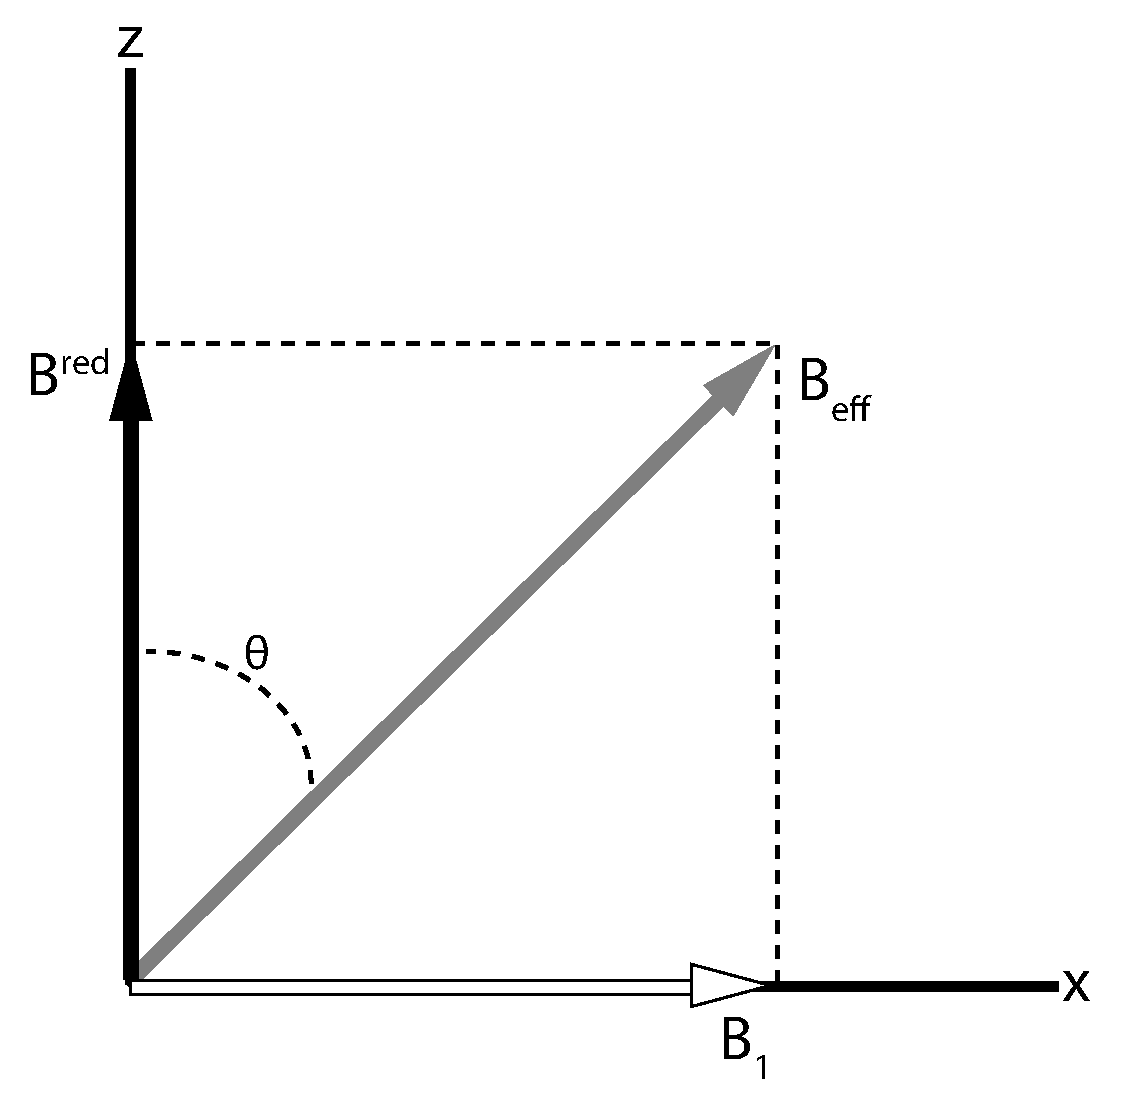
\includegraphics[width=\textwidth, height=7cm, keepaspectratio]{B1Bred.pdf}
  \end{center}
  \caption{In the rotating frame the effective field, $B_{\text{eff}}$, is the vector sum of the reduced field,
  $B_{\text{red}}$ and the $B_1$ field. $\theta$ is the tilt angle defined between $B_{\text{red}}$ and $B_{\text{eff}}$}
  \label{fig:BMag}
\end{figure}


\subsubsection{Pulses}

In NMR experiments pulses are used to manipulate magnetisation in order to obtain a signal. A pulse can be
thought of as a magnetic field oscillating at the frequency of the rotating frame
applied in the $xy$-plane in order to induce procession of the magnetisation. This magnetic field is labelled $B_1$ and is much smaller in amplitude than $B_0$, the actual applied field.

\begin{figure}
  \begin{center}
  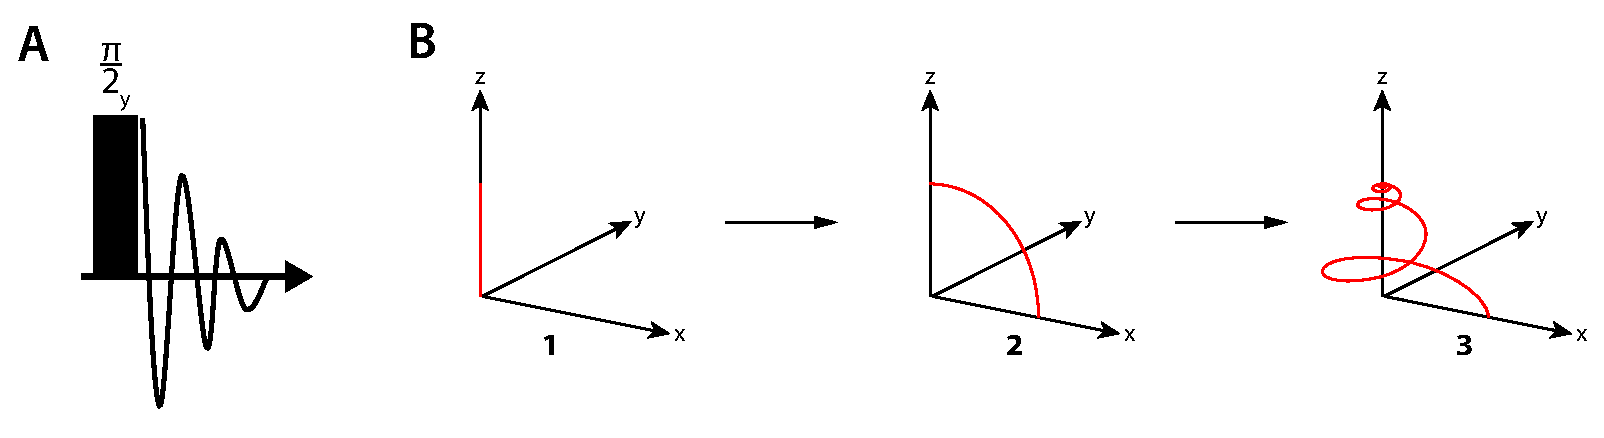
\includegraphics[width=\textwidth]{SpinRelaxation.pdf}
  \end{center}
  \caption{A) A graphical representation used to describe a pulse sequence, the width and height of the block
  refer to the power and duration of pulse respectively, the line represents the acquisition of signal. B)(1) The
  magnetisation lies in equilibrium along the $z$-axis. (2)  The $\pi/2_y$ pulse rotates the magnetisation around the $y$-axis. (3) The magnetisation precesses in the $xy$-plane around the $z$-axis and returns to thermal equilibrium}
  \label{fig:Pulse}
\end{figure}

In the static frame, the magnetisation is processing around $B_0$ at the larmour frequncy, so a relatively weak $B_1$ applied along the $y$-axis, for example, would do little to peturb it, given the effective magnetic field, $B^{\text{eff}}_0$, is calculated by:
\begin{equation}
  B^{\text{eff}}_0 = \sqrt{(B_1)^2+(B_0)^2}
\end{equation}
the much larger $B_0$ dominates here, however, if we apply the $B_1$ in the rotating
frame this becomes
\begin{equation}
  B^{\text{eff}}_0 = \sqrt{(B_1)^2+(B^{\text{red}}_0)^2}
\end{equation}
and using \ref{eqn:redB} as $\omega_{\text{rot}}\rightarrow\omega$, $\Omega\rightarrow0$ and $B^{red}_0\rightarrow0$ so by making the offset small, or zero, the effective field
then lies close to the $xy$-plane and so the magnetisation will be rotated down
from $z$ which is what we'd like to acheive for our experiments.

The key, is that although $B_0$ is much larger than $B_1$, we can still affect magnetisation using $B_1$ by making it oscillate close to the larmour frequency
this is the phenomena of resonance. The angle between $B^{\text{red}}_0$ and $B^{\text{eff}}$ is
called the tilt angle, $\theta$. It can be seen from \fig{fig:BMag} that:
\begin{equation}
\sin(\theta) = \frac{B_1}{B_{\text{eff}}}\qquad\cos(\theta) = \frac{B^{red}_0}{B_{\text{eff}}}\qquad\tan(\theta) = \frac{B_1}{B^{\text{red}}_0}
\end{equation}

These radio frequency (rf) pulses are useful because they can be used to address spins at a specific larmour
frequncy. By applying an rf pulse on resonance with $\ce{^1H}$ we can manipulate the magnetisation of the nuclei whislt not affecting other spins (e.g. $\ce{^13C}$) contained in the sample.

\subsection{Fourier Transform NMR}

In this section we will examine how we can produce an NMR spectrum from the magnetisation of a sample
using the rf pulses we introduced.

In NMR we use a pulse sequence to describe the intensity and duration of pulses used in an
experiment, shown in \fig{fig:Pulse}. The rf pulse, $B_1$, is a $\pi/2$ pulse in the $y$-axis, followed by a signal
acquisition. This pulse tips the magnetisation into the $xy$-plane, and if the pulse length is much less than the
precession period (we will assume so), the spins begin to precess freely around the $z$-axis at the larmour
frequency, $\omega_0$, until they return to the $z$-axis through a process described in \ref{Relaxation}.

In a usual NMR experiment the signal is inductally detected. The oscillation of the spins in the sample induces
a current in the pick-up coils around the sample, which is detected, amplified and transformed into a spectrum.
The resulting free induction decay (FID) is typically an exponentionally decaying sinusoidal function. The signal
produced from this can be written as:
\begin{align}\label{eqn:signal}
  S(t) =& \sum_l s_l(t) \\
  s_l(t) =& a_l\text{exp}\{-(i\omega_l+\lambda_l)t\} = a_l(\cos(\omega_lt) + i\sin(\omega_0t))\text{exp}\{-\lambda_l~t\}
\end{align}
where $S(t)$ is the total signal from from the sample and $s_l$ are the individual spins. Each spin has an amplitude, $a_l$, and an associated decay constant, $\lambda_l$. The nature of which will be discussed in \ref{Relaxation} section. Exponential to trigometric function conversion
is done according to Euler's formula: $\text{exp}\{ix\} = \cos(x) + i\sin(x)$.

$S(t)$ is easy to evaluate and interpret if it originates from one spin or a group of spins precessing
at precisely the same frequency, however, if there are more spins in the sample processing at different frequencies
the FID becomes extremely hard to interpret on its own.

We can clear this picture up however by employing a Fourier transform. This comverts the time-domain data
into the frequncy-domain, such that the total signal in the frequency domain, $S(\omega)$ is the sum of all individual spin signals in the frequency, $S_l(\omega)$:
\begin{equation}
  S(\omega) = \sum_l S_l(\omega)
\end{equation}
This allows us to clearly see which resonances are possessed by our spins in the sample. To
perform a Fourier transform we must do the following:
\begin{equation}
  S_l(\omega) = \int_{0}^{\infty}s_l(t)\text{exp}\{-i\omega t\}dt
\end{equation}
and using \ref{eqn:signal} can be rewritten:
\begin{equation}
  S_l(\omega) = a_l\int_{0}^{\infty}\text{exp}\{(-i(\omega+\omega_l)+\lambda_l t\}dt
\end{equation}
sometimes written more concisely as:
\begin{equation}
  S(\omega) = \mathcal{F}\{S(t)\}(\omega)
\end{equation}
where $S(t)$ is the signal for the time domain (FID) and $S(\omega)$ is the signal in the frequency domain.

The Fourier transform of our general case is:
\begin{equation}
  \mathcal{F}\{S(t)\}(\omega) = a_l\frac{1}{\lambda_l + i(\omega - \omega_l)}
\end{equation}
which is Lorentzian function centered at $\omega_l$ with peak width parameter $\lambda_l$.

The NMR signal represented in the frequency domain is a spectrum. It is usually many peaks
indicating different resonance frequencies of spins in the sample. In the next
section we will discuss chemical shift and J-coupling. Two additional effects that when combined
with larmour frequencies already discussed forms the NMR spectrum as we know it.

\subsection{Chemical Shift and J-coupling}

In a molecule, nuclei are surrounded by clouds of electrons which can shield, or de-sheild, it
from the effects of the external field $B_0$.

The chemical shielding factor, $sigma$, shifts the resonance frequency of the nuclear spin. We
can now include it in \ref{eqn:larmour}:
\begin{equation}
  \omega_j^0 = -\gamma_jB_0(1-\sigma)
\end{equation}
this chemical shielding is specific to each nucleus in the molecule. It is possible
for two or more nuclei to share the same factor. We refer to these as being chemically equivalent.

The shielding is often around $10^-6$ for $\ce{^1H}$. When plotting and examining spectra
it is would not be useful to use absolute frequecies, as discussed they are regualarly in the hundreds of MHz,
whereas the differences in peaks might only be kHz or less. To combat this we use a relative frequency scale
called chemical shift, $\delta$, it is defined as:
\begin{equation}
  \delta = \frac{\omega_j-\omega^\text{ref}_j}{\omega^\text{ref}_j}
\end{equation}
where $\omega_j$ is the precession frequency of the nucleus of interest, and $\omega^\text{ref}_j$ is the precession
frequency of a reference nuclei. $\delta$ is a dimentionless number, unaffected by magnetic field strength, it often
small compared to the size of the field and is reported in parts per million (ppm).

In addition to the external $B_0$ field, the nuclear spins are also affected by the magnetic fields generated
by neighboring spins. These magnetic fields are mediated by the electrons in the chemical bonds. This is refered to as
spin-spin couling or $J$-coupling and gives rise to peak splittings in spectra. These splittings, and therefore the values of $J$-couplings, range from a few Hz to a thousand Hz typically. It is an important factor and is icorperated
in the quatum description on NMR in HAMILTONIAN.

Both of these, $\sigma$ and $J$-couplings, are tensors this means they depend on the orientation of the molecule
and the spin with respect to the magetic field. In liquids, however, tumble rapidly compared to the timescale
of an NMR experiment. This averages the interactions resulting in a scalar quantity for each.

There are additional effects the nuclear spins experience, for example, dipole-dipole coupling which
is a through space spin-spin coupling, and quadrapole coupling where there are spins with >1/2 values
however, these are not relevant to this work.

\subsection{Relaxation}

The last part needed to complete our classical understanding of NMR is relaxation. Relaxation is the process
of the spin returning to the thermal equilibrum. The thermal equilibrium of spin-1/2 nuclei in a
magnetic field is the bulk magnetisation vector pointing in the direction of the $B_0$ field.

In this system there are two forms of relaxation, $T_1$ and $T_2$. $T_1$ is the longitudal relaxation time
constant and $T_2$ is the transverse relaxation time constant the difference between them is shown in \fig{fig:t1t2}.
$T_1$ is the rate constant that governs the return of magnetisation to the $z$-axis from the $xy$-plane. $T_2$ on
the other hand is the time constant that governs the return of magnetisation to equilibrium in the $xy$-plane.
It is more accurate to say that $T_1$ is the relaxation rate constant for populations, and $T_2$ is the relaxation
rate constant coherences, in the density operator (discussed in QUANTUM SECTION). But this is incompatible
with the classical description of NMR.

We can now complete the Bloch equations from \ref{eqn:Bloch}:
\begin{align}
  \frac{dM_x(t)}{dt}\quad=&\quad\gamma(M_y(t)B_z(t)-M_z(t)B_y(t)) - \frac{M_x(t)}{T_2}\\
  \frac{dM_y(t)}{dt}\quad=&\quad\gamma(M_z(t)B_x(t)-M_x(t)B_z(t)) - \frac{M_y(t)}{T_2}\\
  \frac{dM_zt)}{dt}\quad=&\quad\gamma(M_x(t)B_y(t)-M_y(t)B_x(t)) - \frac{M_z(t)-M_0}{T_1}
\end{align}
in order to derive $M_{xy}$ we assume the following:
\begin{equation}
  M_{xy} = M_x + iM_y\qquad\text{and} B_{xy} = B_x + iB_y
\end{equation}
After some algebra we obtain:
\begin{align}
  \frac{dM_xy(t)}{dt}\quad=&\quad-i\gamma(M_{xy}(t)B_z(t)-M_z(t)B_{xy}(t)) - \frac{M_{xy}(t)}{T_2}\\
  \frac{dM_y(t)}{dt}\quad=&\quad~i~\frac{\gamma}{2}(M_{xy}(t)\overline{B_{xy}}(t)-\overline{M_{xy}}(t)B_z(t)) - \frac{M_y(t)}{T_2}\\
\end{align}
where $\overline{M_{xy}} = M_x - iM_y\qquad\text{and} \overline{B_{xy}} = B_x - iB_y$
solving these gives:
\begin{align}
  M_z(t) =& M_{z,\text{eq}} - (M_{z,\text{eq}}-M_z(0))\text{exp}\{\frac{-t}{T_1}\}\\
  M_{xy}(t) =& M_{xy}(0)\text{exp}\{\frac{-t}{T_2}\}
\end{align}

\begin{figure}
  \center{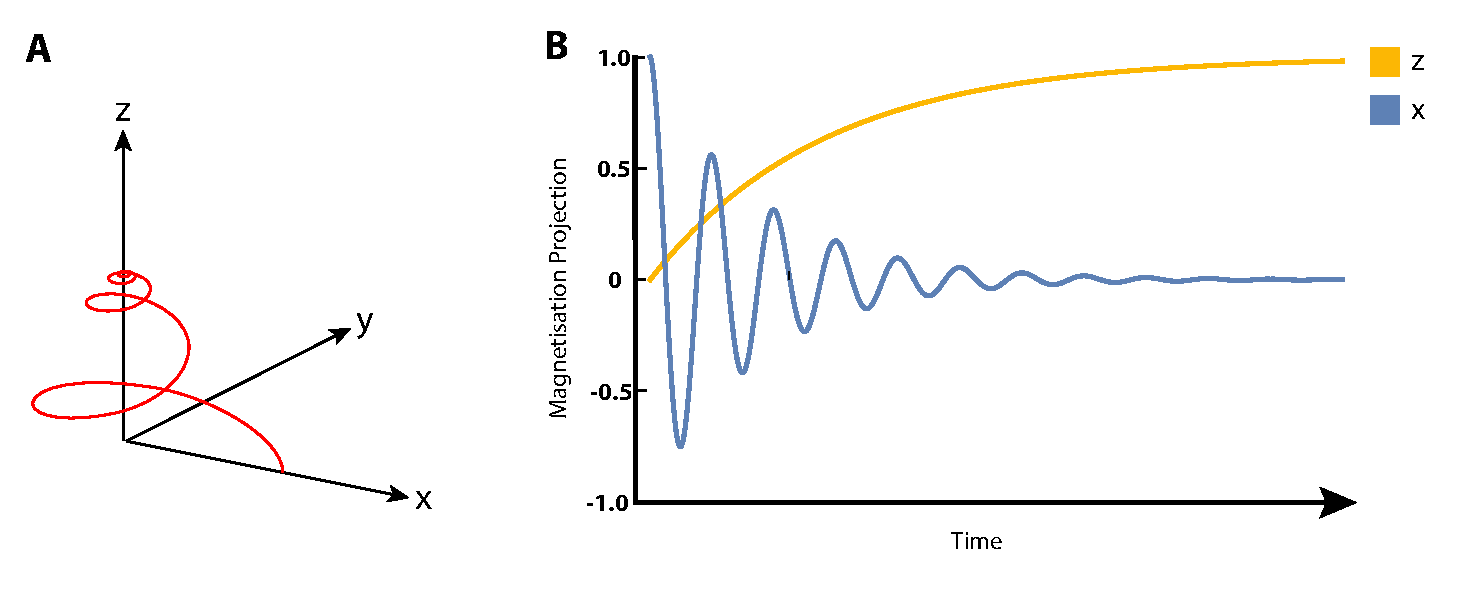
\includegraphics[width=\textwidth]{T1T2.pdf}}
  \caption{A) a magnetisation vector precesses in the $xy$-plane, eventually returning to equilibrium.
  B) A plot of the magnetisation along $z$-axis (yellow) and the $x$-axis (blue) during the relaxation.}
  \label{fig:t1t2}
\end{figure}

Relaxation occurs when the spins exchange energy with their surroundings. They do
this when local magnetic fields, usually caused by the motion of surrounding molecules, oscillate
near the larmour frequency of the relaxing spin. These oscillating fields can be thought of
as local RF pulses we discussed earlier, the key difference is that they only affect a few spins
and not the sample as a whole. Essentially relaxation is an energy exchange between the
spins and the molecules surrounding them. This is the origin of the original name for longitudal
relaxation - spin-lattice relaxation.



\section{Quantum description of NMR}

In this chapter, I will introduce the the quantum description of NMR. Including how
we use operators and superoperators to understand how states change under different conditons and how the energies of the system can be extracted.

\subsection{Nuclear Spin}

Nuclear spin can be treated as a type of angular momentum. Spin angular momentum can be characterized by its total
angular momentum, and the angular momentum with respect to a reference axis (usually z).  Denoted by $\hat{I}$
it is comprised of a magnitude, $\lvert\hat{I}\rvert$, and a direction, $m_I$.
The magnitude is given by
\begin{equation}
  \lvert\hat{I}\rvert = \hbar\sqrt{I(I+1)}
\end{equation}
where $\hbar$ is the reduced Planck constant and $I = 0,\frac{1}{2},1,\dots$. The projection of $\hat{I}$ in
the $z$ direction, $\hat{I}_{z}$, is given by
\begin{equation}
  \hat{I}_{z} = m_I\hbar
\end{equation}
$m_{I}$ can take integer values from $-I$ to $+I$ shown in FIGprojection

For the commonly occuring case of a spin-1/2 nucleus, $I=1/2$ and $m_I = ±1/2$ and if we were to measure $\hat{I}_z$ we would get a value of  with an associated probability depending which state the system is in. Indicating the possible measurement outcomes for $\hat{I}_z$ are $±\frac{\hbar}{2}$.

\begin{figure}
  \begin{center}
  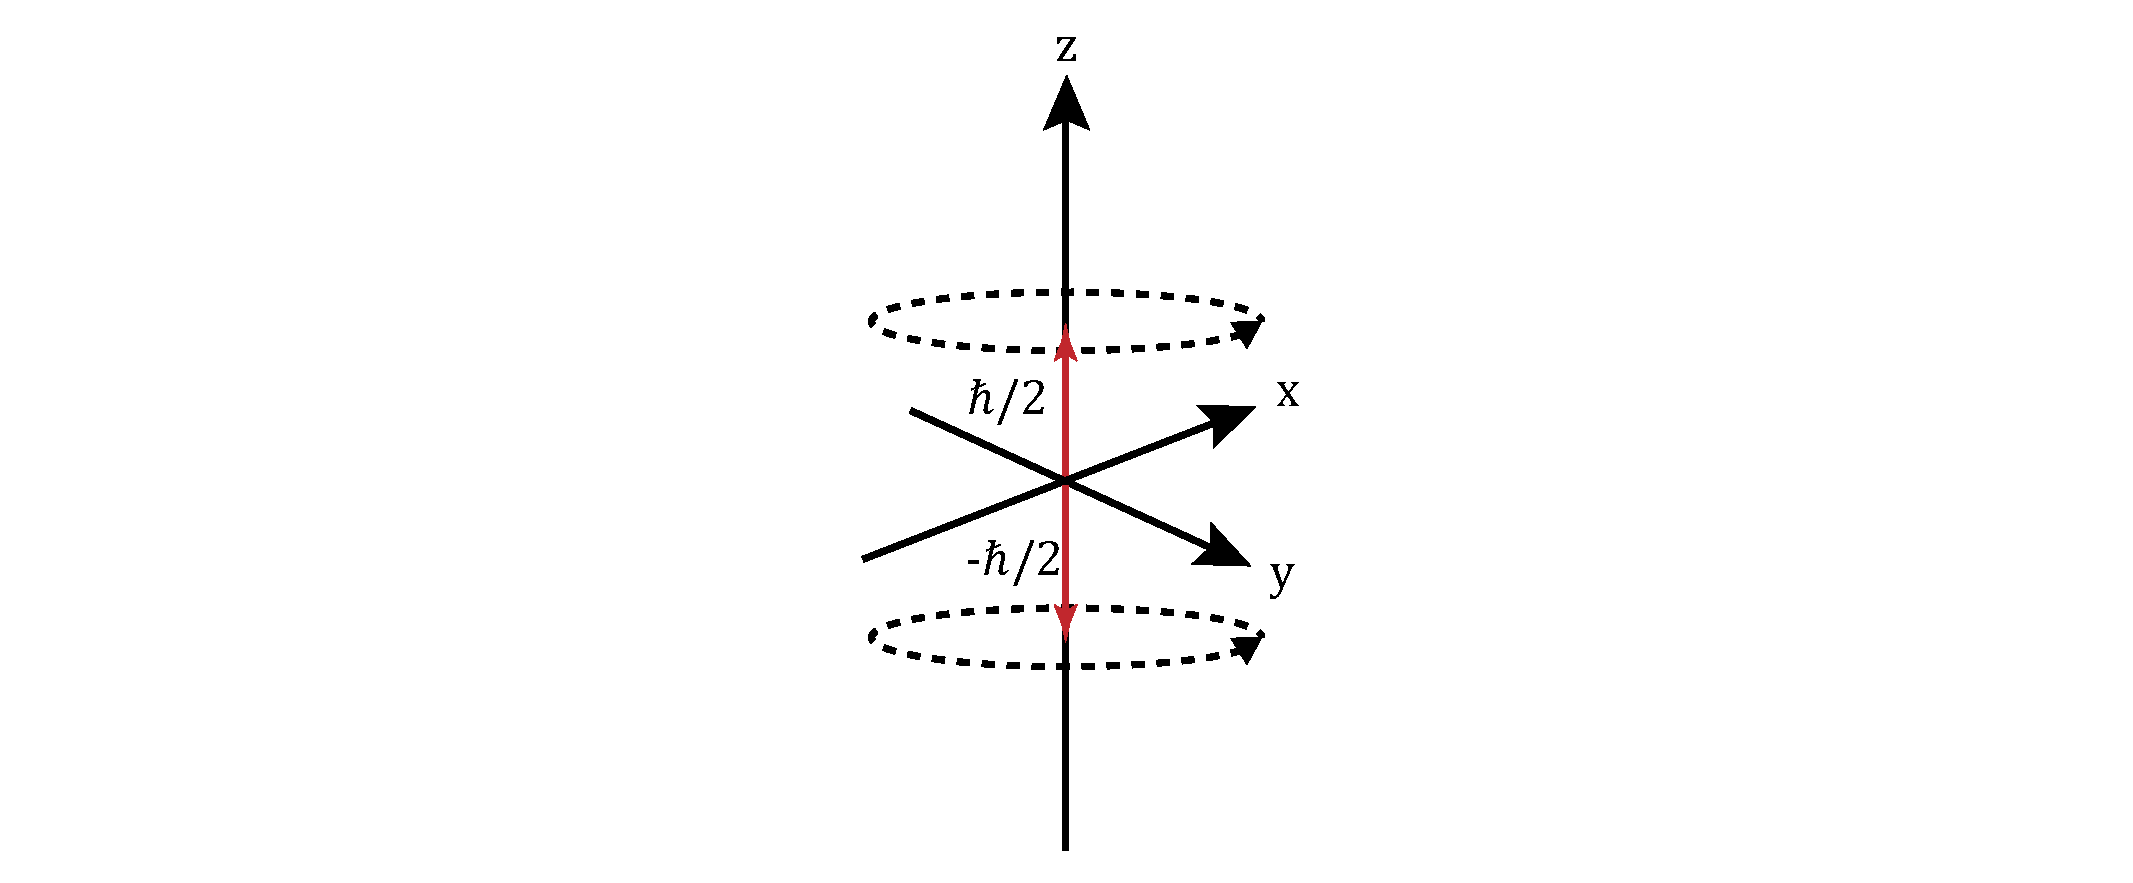
\includegraphics[textwidth=\textwidth,height=5cm,keepaspectratio]{StateProjection.pdf}
  \end{center}
  \caption{The projection of two states in a spin 1/2 nucleus (red arrow) with the magnitudes indicated (black arrow)}
  \label{fig:Projection}
\end{figure}

\subsection{Spin States}

If a spin-1/2 nucleus is placed in a magnetic field (taken to be oriented along $z$) it can be represented using two basis states.
State one has $I = 1/2$, $m_I = 1/2$ and State two has $I = 1/2$, $m_I = -1/2$. We denote these as $\ket{I,m_I}$\citep{dirac_1939}, for simplicity we omit the $I$ and are left with
$\ket{m_I}$. For the special case of a spin-1/2 the two states are known as zeeman states denoted by $\ket{\alpha}$ and $\ket{\beta}$. Where the $\ket{\alpha}$ state has angular momentum +1/2 and $\ket{\beta}$ has -1/2.

The zeeman states take the following form:

\begin{equation}
  \ket{\alpha} = \begin{pmatrix}
    1\\
    0
\end{pmatrix}
 \ket{\beta} = \begin{pmatrix}
   0\\
   1
\end{pmatrix}
\end{equation}

bras are also defined by taking the conjugate transpose of the ket, $\ket{\alpha}^{\dagger} =
\bra{\alpha}$ such that
\begin{equation}
  \bra{\alpha} = \begin{pmatrix}
    1 & 0
\end{pmatrix}
  \bra{\beta} = \begin{pmatrix}
  1 & 0
\end{pmatrix}
\end{equation}

The state, $\ket{\psi}$, of a two level system can now be completely decribed in this basis
as the linear combination of the basis states:
\begin{equation}\label{eqn:zeeman}
  \ket{\psi} = c_1\ket{\alpha} + c_2\ket{\beta} = \begin{pmatrix}
    c_1\\
    c_2
\end{pmatrix}
\end{equation}
\begin{equation}
  \bra{\psi} = c_1^*\bra{\alpha} + c_2^*\ket{\beta} = \begin{pmatrix}
    c_1^* & c_2^*
\end{pmatrix}
\end{equation}

These are normalised such that $c_1c_1^* + c_2c_2^* = 1$.

To complete the picture the sates must me orthonormal. Orthonormality between states exists if
if the inner product of the basis states $\ket{r_i} ~\text{and}~ \ket{r_j}$ satisifies the following conditions:

\begin{equation}
  \langle r_i\vert r_j\rangle = \delta_{ij}
\end{equation}

where the Kronecker delta is:
\begin{equation}
  \delta_{ij} = \begin{cases}
    0 & ~\text{if}~ i \ne j\\
    1 & ~\text{if}~ i = j
                \end{cases}
\end{equation}

where $\langle r_i\vert r_j\rangle = \delta_{ij}$ denotes taking the dot product between the two
vectors $\ket{r_i}$ and $\ket{r_j}$.

The basis states help to quantify the component of a state vector along that state. Take our example from \ref{eqn:zeeman}, we can construct inner products of the overall state, $\ket{\psi}$ with $\ket{\alpha}$ and $\ket{\beta}$ to determine component of the basis states.
\begin{equation}
  \langle\alpha\vert\psi\rangle = c_1 \quad \langle\beta\vert\psi\rangle = c_2
\end{equation}

The outer product of the basis state, $\ket{r_n}$, for an N-spin system must satisfy:
\begin{equation}
  \sum_{n=1}^{N} \ket{r_n}\bra{r_n} = \mathbb{1}
\end{equation}

where $\mathbb{1}$ is an N by N identity matrix.

When a second spin is introduced, the Hilbert space is extended to accommodate additional spin
states by taking the tensor product of the basis states


\begin{align}\label{eqn:2spinstates}
\ket{\alpha_{1}\alpha_{2}} = \ket{\alpha_1} \otimes \ket{\alpha_2} = \begin{pmatrix}
  1\\
  0\\
  0\\
  0
\end{pmatrix} &
\ket{\alpha_{1}\beta_{2}} = \ket{\alpha_1} \otimes \ket{\beta_2} = \begin{pmatrix}
  0\\
  1\\
  0\\
  0
\end{pmatrix}\\
\ket{\beta_{1}\alpha_{2}} = \ket{\beta_1} \otimes \ket{\alpha_2} = \begin{pmatrix}
  0\\
  0\\
  1\\
  0
\end{pmatrix} &
\ket{\beta_{1}\beta_{2}} = \ket{\beta_1} \otimes \ket{\beta_2} = \begin{pmatrix}
  0\\
  0\\
  0\\
  1
\end{pmatrix}
\end{align}
The subscripts indicate which spin we are reffering to, e.g. $\ket{\beta_1\alpha_2}$ means that
spin 1 is in the $\beta$ state and spin 2 is in the $\alpha$ state.

\subsection{Operators}

Operators act on states. To explain this, let's consider a generic operator $\hat{B}$ with eigenstates $\ket{\alpha}$ and $\ket{beta}$. When a state is acted upon by an operator it is denoted by:
\begin{equation}
  \hat{B}\ket{\alpha} = b\ket{\alpha}
\end{equation}

the same state is returned, multiplied by some scalar $b$, that is an eigenvalue of $\ket{\alpha}$
in the operator basis B.

The expectation value of an operator can be found by:
\begin{equation}\label{eqn:expectation}
  \langle\hat{B}\rangle = \langle\alpha\vert\hat{B}\vert\alpha\rangle = b\langle\alpha\vert\alpha\rangle = b
\end{equation}

this returns the eigenvalue.

In NMR we use three operators to determine the projection of angular momentum along a specific axis, $\hat{I}_x$, $\hat{I}_y$, and $\hat{I}_z$. These are defined by the Pauli matrices multiplied by $\frac{\hbar}{2}$.

\begin{equation}
  \hat{I}_x=\frac{\hbar}{2}\begin{pmatrix}
    0 & 1\\
    1 & 0
\end{pmatrix}\quad
\hat{I}_y=\frac{\hbar}{2i}\begin{pmatrix}
  0 & 1\\
  -1 & 0
\end{pmatrix}\quad
\hat{I}_z=\frac{\hbar}{2}\begin{pmatrix}
  1 & 0\\
  0 & 1
\end{pmatrix}
\end{equation}

as an example, let's take the example from before of a spin-1/2 particle in a magnetic field
and see what happens if we were to project the $\ket{\alpha}$ state along the z-axis.
\begin{equation}\label{eqn:operators}
  \hat{I}_z\ket{\alpha} = \frac{\hbar}{2}\begin{pmatrix}
    0 & 1\\
    1 & 0
\end{pmatrix}
\begin{pmatrix}
  1\\
  0
\end{pmatrix} = \frac{\hbar}{2}\begin{pmatrix}
  1\\
  0
\end{pmatrix} = \frac{\hbar}{2}\ket{\alpha}
\end{equation}
We find that $\frac{\hbar}{2}$ is the eigenvalue of $\ket{\alpha}$ for the operator $\hat{I}_z$. For ease of handling in the following examples we will take $\hbar$ = 1.

We will now examine three more operators and explore how they act on states. They are the total square angular momentum, $\hat{I}^2$ and the two shift operators $\hat{I}^+$ and $\hat{I}^-$ defined as the following:

\begin{align}
  \hat{I}^2 =& \hat{I}_x^2 + \hat{I}_y^2 + \hat{I}_z^2\\
  \hat{I}^+ =& \hat{I}_x + i\hat{I}_y\\
  \hat{I}^- =& \hat{I}_x - i\hat{I}_y
\end{align}
They act on states according to:
\begin{align}
  \hat{I}^2\ket{I,m_I} =& I(I+1)\ket{I, m_I}\\
  \hat{I}^+\ket{I,m_I} =& \sqrt{(I(I+1)-m_I(m_I+1))}\ket{I,m_{I+1}}\\
  \hat{I}^-\ket{I,m_I} =& \sqrt{(I(I+1)-m_I(m_I-1))}\ket{I,m_{I-1}}
\end{align}
Using a spin-1/2 particle in a magnetic field as an example we'll let these operators act on the $\ket{\alpha}$ state
\begin{align}
  \hat{I}^2\ket{\alpha} =& \frac{3}{4}\ket{\alpha}\\
  \hat{I}^+\ket{\alpha} =& 0\\
  \hat{I}^-\ket{\alpha} =& \ket{\beta}\\
  \hat{I}^+\ket{\beta} =& \ket{\alpha}\\
  \hat{I}^-\ket{\beta} =& 0
\end{align}
As the '+' and '-' denote raising or lowering $m_I$ by 1


We can see if two operators commute by using the commutator which is defined as:
\begin{equation}
  [\hat{A},\hat{B}] = \hat{A}\hat{B} - \hat{B}\hat{A}
\end{equation}

If $[\hat{A},\hat{B}] = 0$ the operators are said to commute. The $\hat{I}_z$, $\hat{I}_z$ and $\hat{I}_z$
have cyclic commutation rules:
\begin{align}\label{eqn:commutator}
  [\hat{I}_x,\hat{I}_y] = i\hat{I}_z\\
  [\hat{I}_y,\hat{I}_z] = i\hat{I}_x\\
  [\hat{I}_x,\hat{I}_z] = i\hat{I}_y
\end{align}

These relationships are important in NMR as they help govern the rules for the rotations of spins.

\subsection{Superoperators}

Like states, that can be transformed by operators, we can define objects that act in a similar manner on operators. These objects are called superoperators.

To start, let's take a simple commutation superoperator, $\hat{\hat{A}}$, defined as:
\begin{equation}
  \hat{\hat{A}}\hat{B} = [\hat{A},\hat{B}] = \hat{A}\hat{B} - \hat{B}\hat{A}
\end{equation}
Applying it to operator $\hat{B}$ results in the commutation of $\hat{A}$ and $\hat{B}$

In NMR, three rotational superoperators can be defined using the commutation superoperators from \ref{eqn:operators}:
\begin{equation}
 \hat{\hat{R}}_x(\theta) = \text{exp}\{-i\hat{\hat{I}}_x\theta\}\quad\hat{\hat{R}}_y(\theta) = \text{exp}\{-i\hat{\hat{I}}_y\theta\}\quad\hat{\hat{R}}_z(\theta) = \text{exp}\{-i\hat{\hat{I}}_z\theta\}
\end{equation}

These are applied to to the angular momentum operators using the sandwich formula:
\begin{equation}
  \hat{\hat{R}}_x(\theta)\hat{I}_z = \text{exp}\{-i\hat{\hat{I}}_x\theta\}\hat{I}_z\text{exp}\{+i\hat{\hat{I}}_x\theta\}
\end{equation}

The result of this is a rotation of $\hat{I}_z$ around the $x$-axis by an angle $\theta$:
\begin{equation}
  \hat{\hat{R}}_x(\theta)\hat{I}_z = \cos{\theta}\hat{I}_z - \sin{\theta}\hat{I}_y
\end{equation}

The rotational direction (sign of the $\sin{\theta}$ term) is determined by the right hand co-ordinate system defined in \ref{eqn:commutator}.

We will now discuss how these are used in describing the spin dynamics of a spin system.

\subsection{Density Operator}

The density operator gives us information on the state of groups of spins in a spin system.

Let's go back once again to a spin-1/2 particle in a magnetic field. Where $\ket{\psi}$ is some superposition state in the two level system such that:
\begin{align}
\ket{\psi} =& \begin{pmatrix}
    c_1\\
    c_2
\end{pmatrix} = c_1\ket{\alpha} + c_2\ket{\beta}\\
\bra{\psi} =& \begin{pmatrix}
  c_1^* & c_2^*
\end{pmatrix} = c_1^*\bra{\alpha} + c_2^*\bra{\beta}
\end{align}

The density operator has the form:
\begin{equation}
  \hat\rho = \overline{\ket{\psi}\bra{\psi}} = \begin{pmatrix}
    c_1c_1^* & c_1c_2^*\\
    c_2c_1^* & c_2c_2^*
\end{pmatrix}
\end{equation}

If the number of spins is increased, the denstiy operator's form does not change instead it provides
an average fo the entire group of spin states. The population of a given state is given by the expectation value of the density operator as in \ref{eqn:expectation}. If we would like to know
the population of state $\ket{\alpha}$ we would perform the following:
\begin{equation}
  \langle\alpha\vert\hat\rho\vert\alpha\rangle = \langle\alpha\vert\psi\rangle \langle\alpha\vert\psi\rangle = c_1^*c_1
\end{equation}

The diagonal elements of $\hat\rho$ are state populations or the probabilities of being in a certain state.

The off-diagonal elements are coherences between states. These coherences are complex numbers and two coherences between the same pair of states are complex cojugates of each other. e.g.:
\begin{equation}
  \langle\alpha\vert\hat\rho\vert\beta\rangle = (\langle\beta\vert\hat\rho\vert\alpha\rangle)^* = c_1c_2^* = (c_1^*c_2)^*
\end{equation}
The coherence order between two states in a magnetic field is defined as the difference in angular
momentum projection along the $z$ axis. In our two spin this would be(with $\hbar = 1$):
\begin{align}
  \hat{I}_z\ket{\beta} = m_\alpha = +\frac{1}{2}\ket{\alpha}\\
  \hat{I}_z\ket{\beta} = m_\beta = -\frac{1}{2}\ket{\beta}
\end{align}
We can use these results to calculate the coherence order of the coherence $\langle\alpha\vert\hat\rho\vert\beta\rangle$:
\begin{equation}
 m_\alpha - m_\beta = +1
\end{equation}
and conversely the coherence order of $\langle\beta\vert\hat\rho\vert\alpha\rangle$ is:
\begin{equation}
  m_\beta - m_\alpha = -1
\end{equation}

Now let's look at how $\hat\rho$ relates to the angular momentum operators give in \ref{eqn:operators}.

Usually in NMR there are $>10^{20}$ spins in the sample, the density operator becomes more advantageous here
as mentioned it contains information about the entire spin ensemble. Normally, there is only a small population difference between $\alpha$ and $\beta$ (see \ref{Population}),
but for this example let's imagine we have found a sufficiently strong enough field for a population difference of $0.1$. The density operator in this case would be:
\begin{equation}
  \hat\rho = \frac{1}{2}\begin{pmatrix}
    1 + 0.1 & 0\\
    0 & 1-0.1
\end{pmatrix}
\end{equation}
using the definition given in \ref{eqn:operators} we can re-write this as
\begin{equation}
  \hat\rho = \frac{1}{2}\hat{\mathbb{1}} + 0.1\hat{I}_z
\end{equation}
$\hat{\mathbb{1}}$ is identity matrix and corresponds to no population difference between $\ket{\alpha}$ and $\ket{\beta}$.

$\hat{\mathbb{1}}$ is unaffected by rotations so can be ignored in the context of NMR
and so we write
\begin{equation}
  \hat{\rho} = 0.1\hat{I}_z
\end{equation}
to describe the $z$ magnetisation of our sample.

The density operator can also be used to to describe the evolution of a spin system under operations. If we applied a $90$ degree pulse along the $y$ axis, denoted using radians by $(\pi/2)_y$. That is the equivalent of propagating the initial density operator, $\rho_0$
under the rotation superoperator $\hat{\hat{R}}_y(\pi/2)$:
\begin{equation}
  \hat{\rho}_1 = \hat{\hat{R}}_y(\frac{\pi}{2})\hat\rho_0 = \text{exp}\{-i(\frac{\pi}{2})\hat{\hat{I}}_y\}\hat{I}_z\text{exp}\{+i(\frac{\pi}{2})\hat{\hat{I}}_y\} = \hat{I}_x
\end{equation}
Now the magnetisation is in the $x$-axis it will begin to precess about the $z$-axis which using our notation is the equivalent of of propagating $\hat{I}_x$ ($\hat{\rho}_1$)
under $\hat{\hat{R}}_z(\omega t)$:
\begin{align}\label{eqn:propagate}
  \hat{\rho}_2 = \hat{\hat{R}}_z(\omega t)\hat{\rho}_1 =& \text{exp}\{-i\omega t\hat{\hat{I}}_z\}\hat{I}_x\text(exp)\{+i\omega t\hat{\hat{I}}_z\}\\
   =& \cos(\omega t)\hat{I}_x + \sin(\omega t)\hat{I}_y
\end{align}
where $\omega$ is the larmour frequency, and $t$ is time.

the $\text{exp}\{i\omega t\}$ is called a propagator, because it propagates the density operator in time.

The Hamiltonian, the energy operator, describes how the system evolves in time and uses progators, rotational superoperators and the density operator in order to do so.

\subsection{The Hamiltonian}

As mentioned the Hamiltonian is the energy operator. It provides information on the enrgies of states in a system.

If we let $\ket{\psi_1}$ and $\ket{\psi_2}$ be eigenstates of the Hamiltonian $\hat{H}$ then
\begin{align}
  \hat{H}\ket{\psi_1} = E_1\ket{\psi_1}\\
  \hat{H}\ket{\psi_2} = E_2\ket{\psi_2}
\end{align}

The Hamiltonian can also be expressed in matrix form:
\begin{equation}
  \hat{H} = \begin{pmatrix}
    E_1 & 0\\
    0 & E_2
\end{pmatrix}
\end{equation}
If the Hamiltonian is written in the eigenbasis of the system its main diagonal correspond to state energies and it has values of $0$ everywhere else.

The evolution in time of a quantum system is described by the Schr\"odinger equation:
\begin{equation}
  i\hbar\frac{\partial}{\partial{t}}\ket{\psi} = \hat{H}\ket{\psi}
\end{equation}
The $\hbar$ was included for completeness sake and will again be set to equal $1$.

In NMR we describe the dynamics of a system using the density operator evolution rather than the evolution of the states using
\begin{align}
  \frac{\partial}{\partial{t}}\ket{\psi} = -i\hat{H}\ket{\psi}\\
  \frac{\partial}{\partial{t}}\bra{\psi} = i\bra{\psi}\hat{H}
\end{align}

we can derive\citep{Neumann2018}:
\begin{align}
  \frac{\partial}{\partial{t}}\hat\rho\quad=&\quad \frac{\partial}{\partial{t}}[\ket{\psi}\bra{\psi}]\\
  =&\quad[\frac{\partial}{\partial{t}}\ket{\psi}]\bra{\psi} + \ket{\psi}[\frac{\partial}{\partial{t}}\bra{\psi}]\\
  =&\quad-i\hat{H}\ket{\psi}\bra{\psi} + i\ket{\psi}\bra{\psi}
\end{align}
to give the relationship
\begin{equation}
  \frac{\partial}{\partial{t}}\hat\rho = -i[\hat{H},\hat\rho]
\end{equation}
this is called the Louisville von Neumann equation.

Returning to our spin-1/2 particle in a magnetic field. The Hamiltonian is initially
proportional to the $z$ angular momentum operator
\begin{equation}
  \hat{H} = \omega\hat{I}_z
\end{equation}

where $\omega = -\gamma B_0$. In matrix form, in our original zeeman basis, the Hamiltonian is:
\begin{equation}
  \hat{H} = \begin{pmatrix}
+\frac{\omega}{2} & 0\\
0 & -\frac{\omega}{2}
\end{pmatrix}
\end{equation}
where
\begin{equation}
  \hat{H}\ket{\alpha} = +\frac{\omega}{2}\ket{\alpha}
\end{equation}

The density operator evolves under a Hamiltonian like so:
\begin{equation}
  \hat\rho(t) = \text{exp}\{-i\hat{H}t\}\hat\rho(0)\text{exp}\{+i\hat{H}t\}
\end{equation}

In \ref{eqn:propagate}, we saw that the precession of a spin-1/2 particle in a magnetic field can be described using the rotation superoperator around the $z$-axis $\hat{\hat{R}}_z(\omega t)$. We know that for this system its analagous to $\hat{H} = \omega\hat{I}_4$.

If the density operator commutes with the Hamiltonian there is no evolution of the system
this can be seen more clearly using propagators with $\hat{H} = \omega\hat{I}_z$ and $\rho(0) = \hat{I}_z$
\begin{equation}
  \rho(t) = \text{exp}\{-i\omega t\hat{\hat{I}}_z\}\hat{I}_z\text{exp}\{+i\omega t\hat{\hat{I}}_z\} = \hat{I}_z
\end{equation}
If the density operator does not commute with the Hamiltonian it will evolve. To demostrate this we use $\hat{H} = \omega\hat{I}_z$ as before  however this time $\hat\rho(0) = \hat{I}_x$
\begin{equation}
  \hat\rho(t) = \text{exp}\{-i\omega t\hat{\hat{I}}_z\}\hat{I}_x\text{exp}\{+i\omega t\hat{\hat{I}}_z\} = \cos(\omega t)\hat{I}_x + \sin(\omega t)\hat{I}_y
\end{equation}
The Hamiltonian for multi-spin system is slightly more complicated. Consider a two spin
system $I_1$ and $I_2$ with $J$-coupling $J_{12}$ the Hamiltonian then becomes:
\begin{equation}
  \hat{H} = \omega_1\hat{I}_1 + \omega_2\hat{I}_2 + 2\pi J_{12}\hat{\mathbf{I}}_1.\hat{\mathbf{I}}_2
\end{equation}
where $\hat{\mathbf{I}}_1.\hat{\mathbf{I}}_2 = \hat{I}_{1x}\hat{I}_{2x} + \hat{I}_{1y}\hat{I}_{2y} + \hat{I}_{1z}\hat{I}_{2z}$.
In matrix form in the zeeman basis this is:
\begin{equation}
  \hat{H} = \frac{1}{2}\begin{pmatrix}
    +\omega_1 + \omega_2 + \pi J_{12} & 0 & 0 & 0\\
    0 & +\omega_1 - \omega_2 - \pi J_{12} & 2\pi J_{12} & 0\\
    0 & 2\pi J_{12} & -\omega_1 + \omega_2 - \pi J_{12} & 0\\
    0 & 0 & 0 & -\omega_1 - \omega_2 - \pi J_{12}
\end{pmatrix}
\end{equation}

The zeeman basis is no longer an eigenbasis of the Hamiltonian because the $J$-coupling
introduces off-diagonal terms. In practice, when $|\omega_1-\omega_2| >> 2\pi J_{12}$
these terms are ignored because the zeeman basis is approxiamely the eigen basis of the Hamiltonian. This is termed the secular approxiamation.

However, when this is not the case, the Hamiltonian requires diagonalisation which is beyond the scope of this introduction but will be addressed if needed in later chapters.
